\section*{Process}
Processen er bevidst opdelt i kategorier, der eksekveres med tidsmæssigt
overlap. Ideen er at starte med at skære alt massiv træ op på råmål tidligt,
samt stavlime hvor nødvendigt. Derefter udføres arbejde med pladematerialer og
finer. Udskæring på finmål af de opskårede emner udskydes til de hver i sær skal
bruges. Denne fremgang forlænger den tilgængelige tid til akklimatisering af
træet, mht. Værkstedets luftfugtighed, uden at forsinke arbejdet.

Udoveer diverse opstillinger, bruges der to skabeloner i projektet, begge til
benene. En skabelon bruges til tapering, og en til udfræsningen i toppen.

\begin{figure}[htb]
\centering
\fbox{
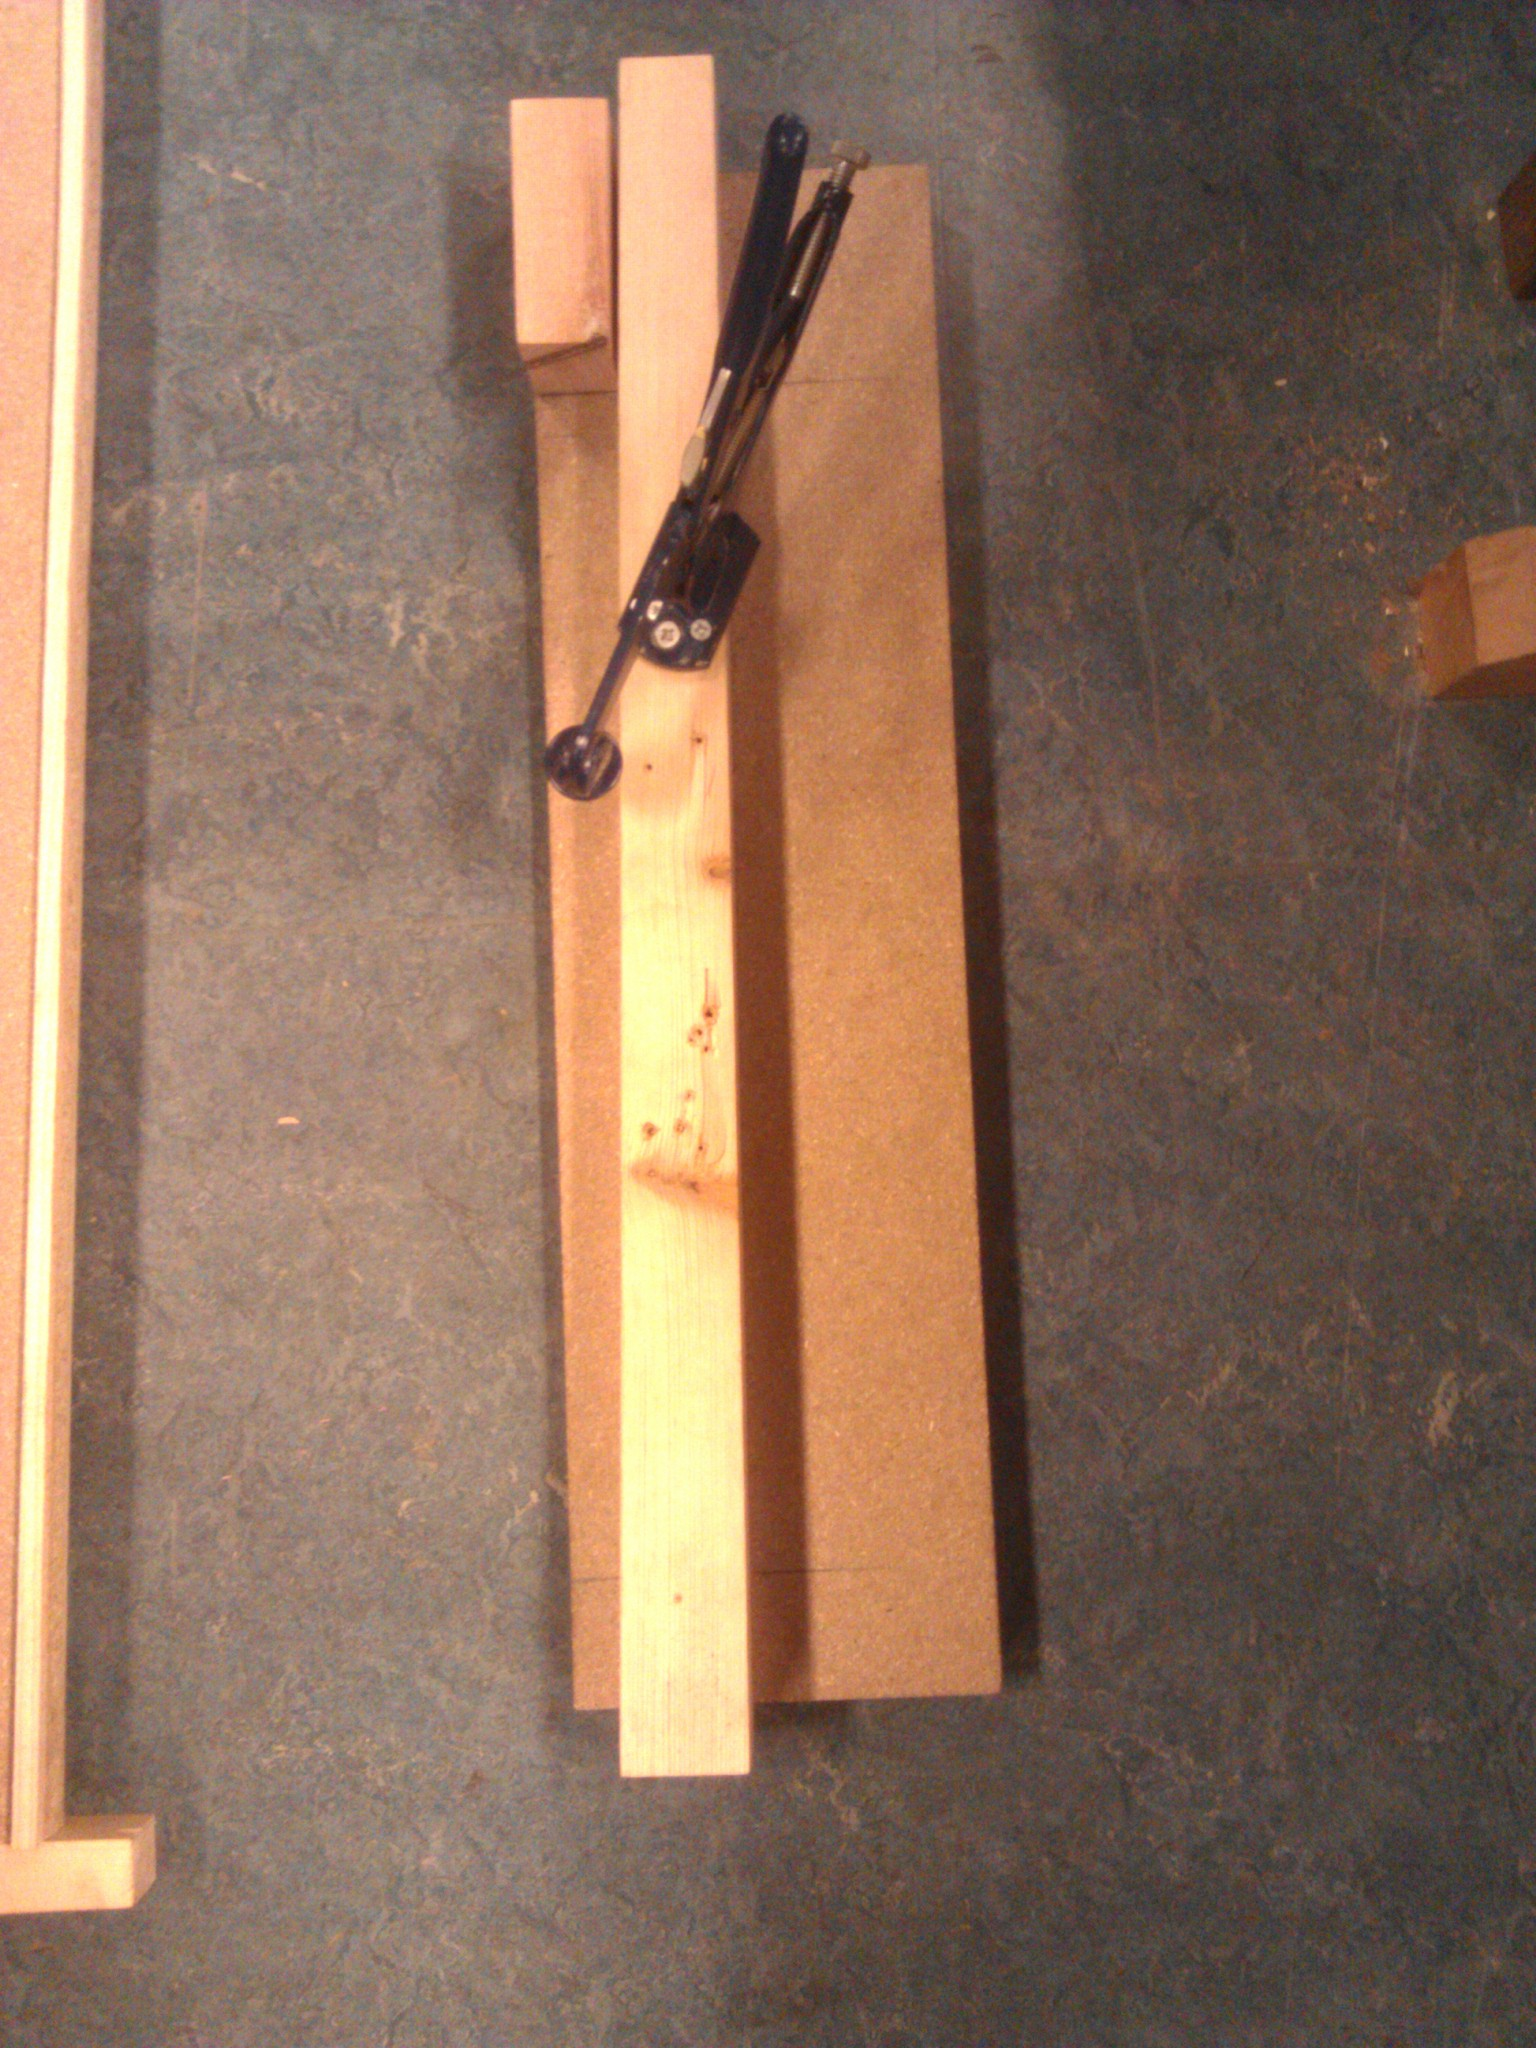
\includegraphics[width=0.4 \textwidth]{imgs/skabelon-tapering.jpg}
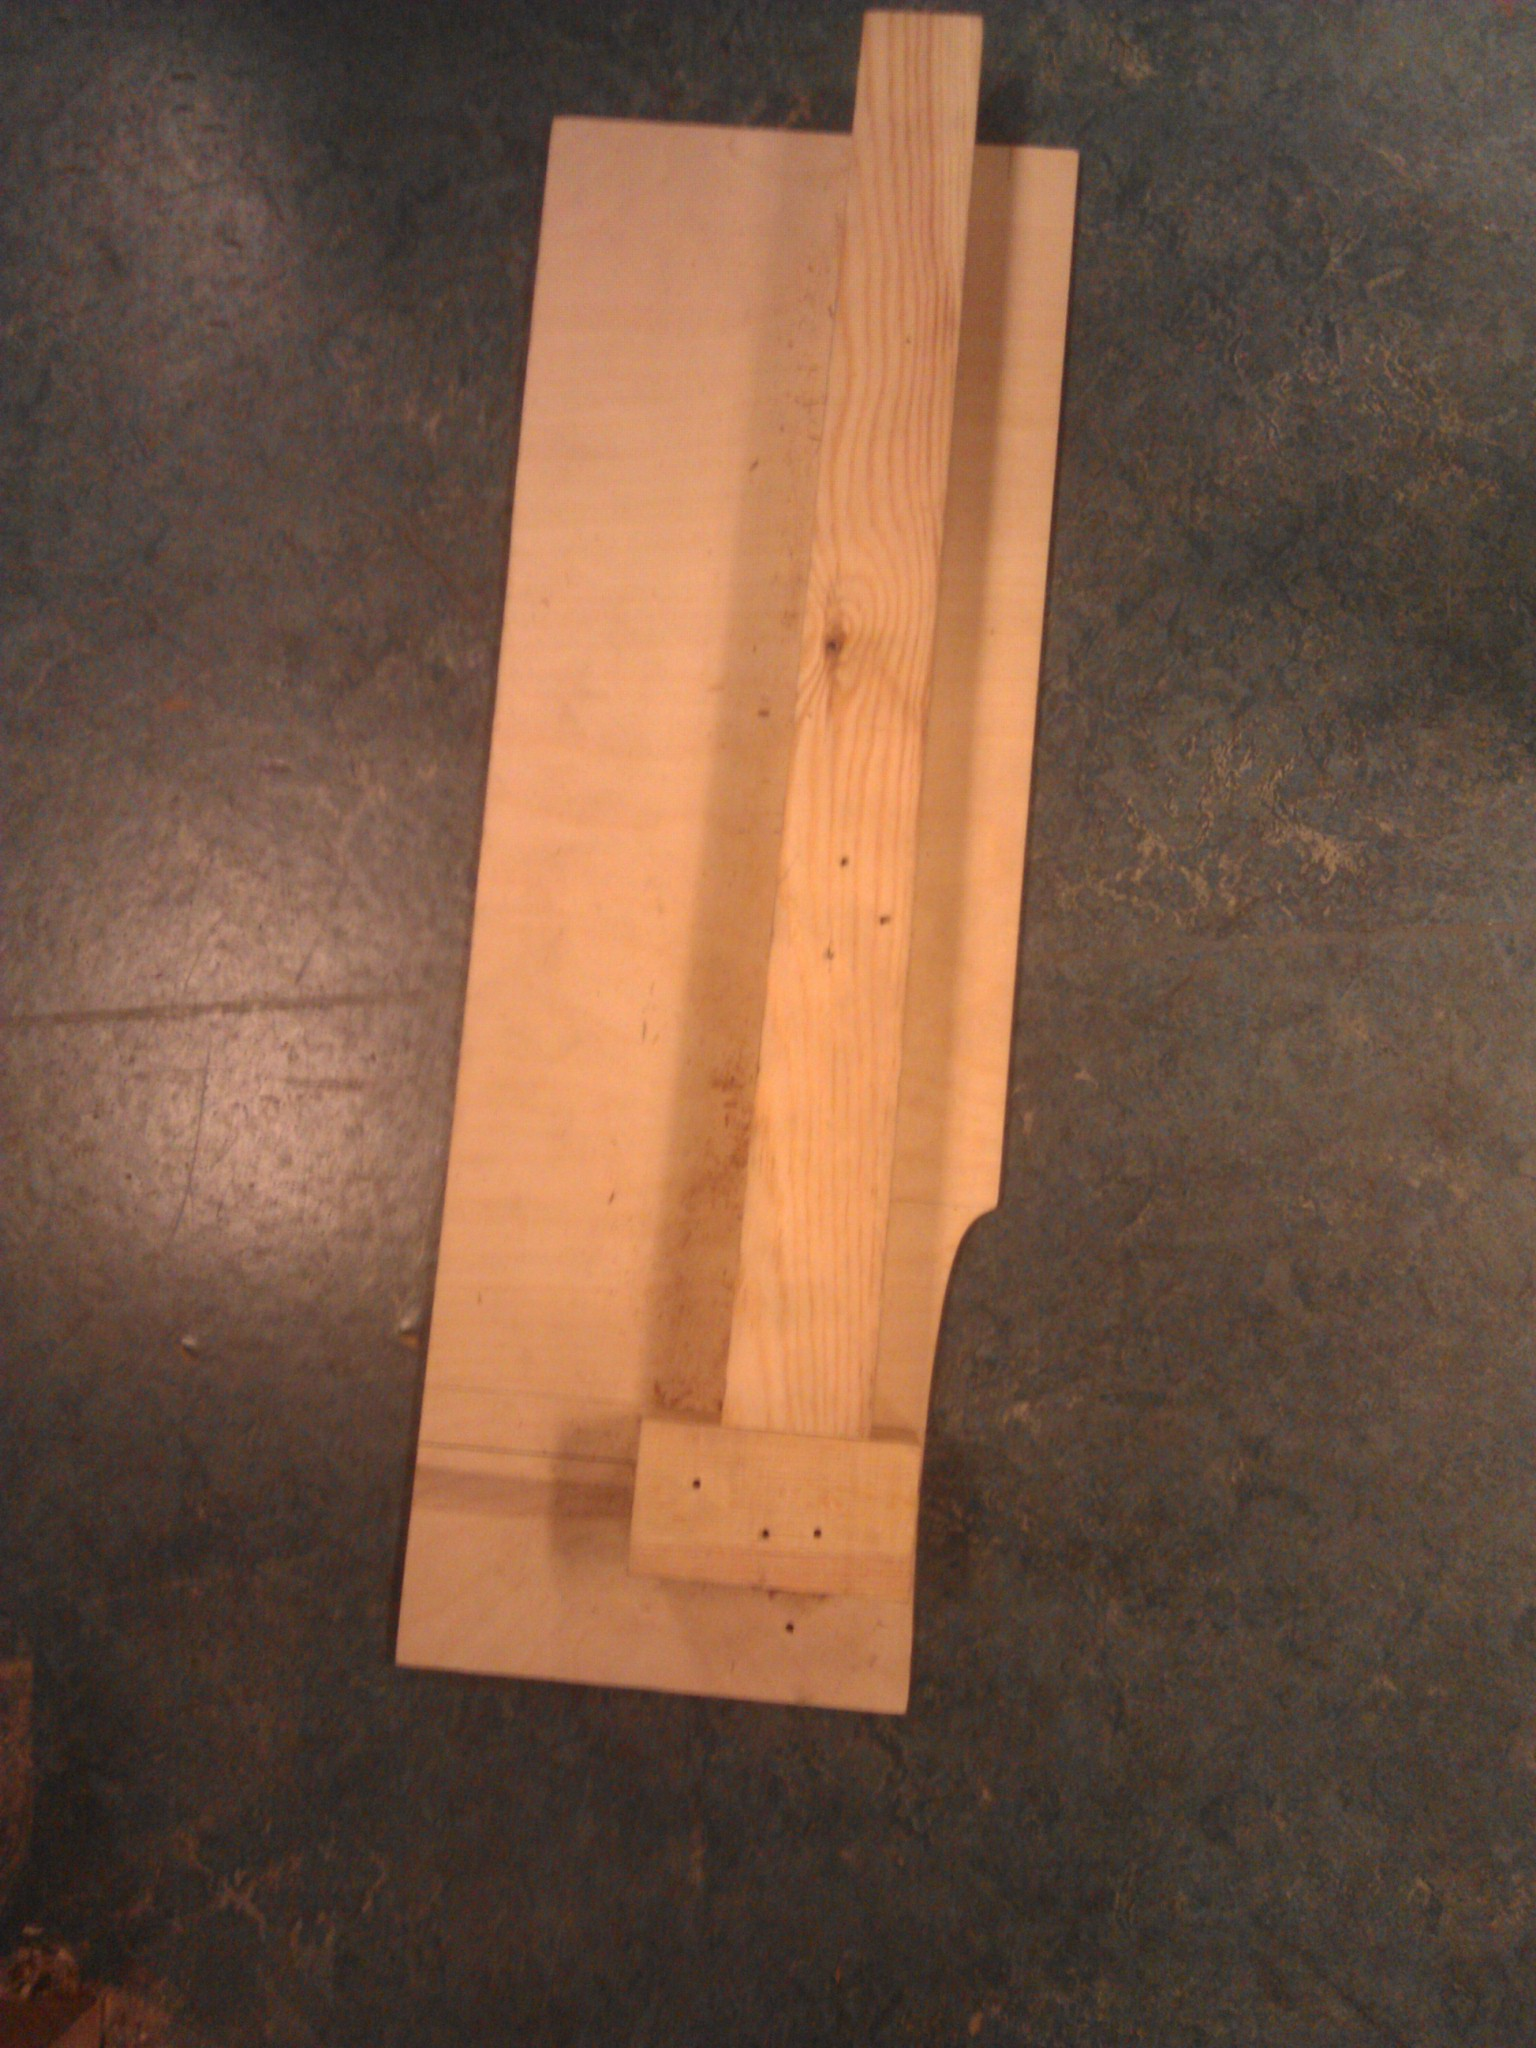
\includegraphics[width=0.4 \textwidth]{imgs/skabelon-fraesning.jpg}
}
\caption{Skabelon til tapering af ben (vesntre). Skabelon til udfræsning (højre)}
\end{figure}

\subsection*{Overfladebehandling}
